\begin{figure}[t]
  \centering
  \pgfplotsset{  
    scale only axis,
%    xmin=1,
  }
  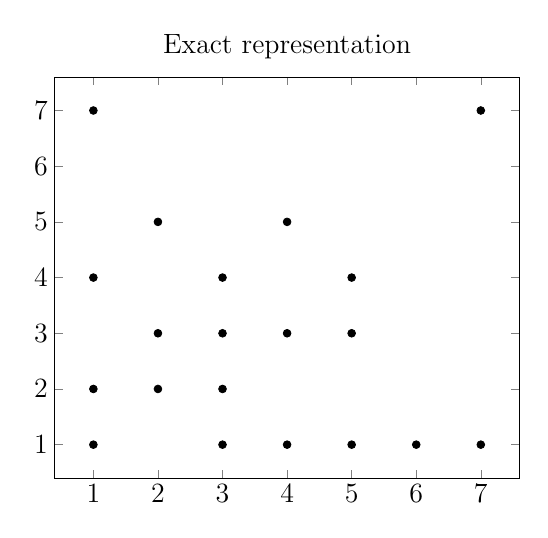
\begin{tikzpicture} [scale=0.7, font=\Large]
    \begin{axis}[
        title=Exact representation,
        xtick=data,
%        ymin=0,
      ]
      \addplot[black, mark=*, only marks]
       plot coordinates
       {  
       (1,1)       (3,1) (4,1) (5,1) (6,1) (7,1)
       (1,2) (2,2) (3,2) 
             (2,3) (3,3) (4,3) (5,3)
       (1,4)       (3,4)       (5,4)
             (2,5)        (4,5) 
       (1,7)                               (7,7)
       }; 
    \end{axis}
  \end{tikzpicture}
  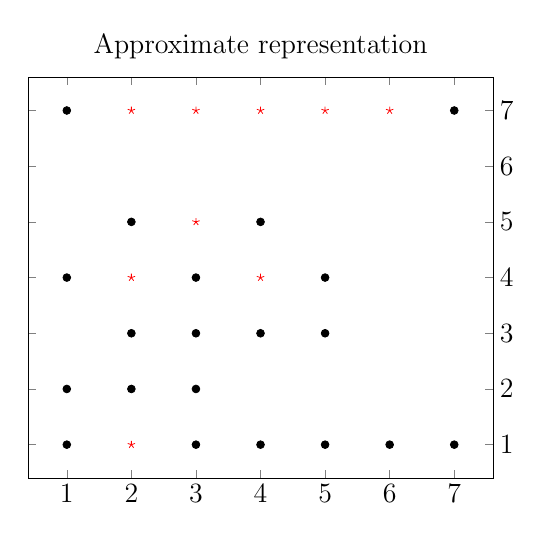
\begin{tikzpicture} [scale=0.7, font=\Large]
    \begin{axis}[
        yticklabel pos=right,
        xtick=data,
        title=Approximate representation
        ]
      \addplot[black, mark=*, only marks]
       plot coordinates
       {  
       (1,1)       (3,1) (4,1) (5,1) (6,1) (7,1)
       (1,2) (2,2) (3,2) 
             (2,3) (3,3) (4,3) (5,3)
       (1,4)       (3,4)       (5,4)
             (2,5)        (4,5) 
       (1,7)                               (7,7)
       }; 
      \addplot[red, mark=star, only marks]
       plot coordinates
       {  
             (2,1) 
       


                  (2,4)    (4,4)
                       (3,5)
            (2,7) (3,7) (4,7) (5,7) (6,7)
       }; 

    \end{axis}
  \end{tikzpicture}

 \caption{Comparison between an exact and an approximate representation of the same domain. The stars are values that should not be there, but the approximate representation only stores the boundaries for the second dimension.}\label{fig:pair}
\end{figure}
